%%
%% This is file `article.tex',
%%
%% Commands for TeXCount
%TC:macro \cite [option:text,text]
%TC:macro \citep [option:text,text]
%TC:macro \citet [option:text,text]
%TC:envir table 0 1
%TC:envir table* 0 1
%TC:envir tabular [ignore] word
%TC:envir displaymath 0 word
%TC:envir math 0 word
%TC:envir comment 0 0
%%
%%
%% The first command in your LaTeX source must be the \documentclass command.
\documentclass[sigconf, nonacm]{acmart}

%%
%% \BibTeX command to typeset BibTeX logo in the docs
\AtBeginDocument{%
  \providecommand\BibTeX{{%
    \normalfont B\kern-0.5em{\scshape i\kern-0.25em b}\kern-0.8em\TeX}}}

%% Rights management information.  This information is sent to you
%% when you complete the rights form.  These commands have SAMPLE
%% values in them; it is your responsibility as an author to replace
%% the commands and values with those provided to you when you
%% complete the rights form.
\setcopyright{rightsretained}
\copyrightyear{2021}
%\settopmatter{printccs=true, printacmref=true}

\usepackage{listings}
\usepackage{makecell}
\usepackage{tabularx}

%%
%% end of the preamble, start of the body of the document source.
\begin{document}

\title{Literature review of Formal Methods applied to Blockchain technology}

\author{Henoch Vitureira}
\affiliation{%
  \institution{Instituto Politécnico de Setúbal}
  \streetaddress{Campus do IPS - Estefanilha, 2910-761}
  \city{Setúbal}
  \country{Portugal}}
\email{2016041081@estudantes.ips.pt}


%%
%% By default, the full list of authors will be used in the page
%% headers. Often, this list is too long, and will overlap
%% other information printed in the page headers. This command allows
%% the author to define a more concise list
%% of authors' names for this purpose.
\renewcommand{\shortauthors}{Henoch Vitureira}

%%
%% The abstract is a short summary of the work to be presented in the
%% article.
\begin{abstract}
  Lorem ipsum dolor sit amet, consectetur adipiscing elit. 
  Vestibulum enim nibh, aliquet sit amet ex suscipit, efficitur fringilla enim. 
  Vestibulum elementum fringilla sodales. Cras malesuada sollicitudin consectetur.
  Cras elit nibh, tempus elementum dui vitae, sagittis porttitor elit. In sollicitudin purus neque, eu tristique felis varius in. Morbi sed commodo eros.
  Pellentesque ornare sed felis et bibendum.
\end{abstract}

%%
%% The code below is generated by the tool at http://dl.acm.org/ccs.cfm.
%% Please copy and paste the code instead of the example below.
%%
\begin{CCSXML}
  <ccs2012>
  <concept>
  <concept_id>10011007.10011074.10011099.10011105</concept_id>
  <concept_desc>Software and its engineering~Process validation</concept_desc>
  <concept_significance>500</concept_significance>
  </concept>
  <concept>
  <concept_id>10002978.10002979</concept_id>
  <concept_desc>Security and privacy~Cryptography</concept_desc>
  <concept_significance>500</concept_significance>
  </concept>
  </ccs2012>
\end{CCSXML}

\ccsdesc[500]{Software and its engineering~Process validation}
\ccsdesc[500]{Security and privacy~Cryptography}

%%
%% Keywords. The author(s) should pick words that accurately describe
%% the work being presented. Separate the keywords with commas.
\keywords{Software Quality, Formal Methods, Blockchain, Smart contracts}


%%
%% This command processes the author and affiliation and title
%% information and builds the first part of the formatted document.
\maketitle

\section{Introduction}
The rising complexity of features offered by software gives us the ability to use it for the most integrity and reliability dependent needs of our lives. 
Information systems that rely on these base principles can be financial and health related services, and in most recent times, blockchain based applications. 
Blockchain, being a decentralized and distributed network protocol that can be used as the core of a monetary system that performs peer-to-peer transactions, 
it needs the assurance of coordination and consensus of its economy’s state~\cite{Duan2018}. 
Knowing that the protocol of a given blockchain project is what dictates how transactions and their coordination is maintained, the assurance of security and safety is a given. 
Formal methods can be introduced in order to provide unequivocal evidence that a given blockchain system and its consensus algorithm are secure and in according to expected software quality.

Formal methods are a rigorous description of a system or process using mathematics that aims to provide evidence of its reliability and robustness, 
according the specification in question~\cite{Regan2014}.

Contrasting with normal testing, formal verification is performed during the design process, it ensure the design is correct and allows the verification
of any situation, while regular testing cannot test for every possible input~\cite{Murray2019}.

This paper is organized as follows. Section \ref{formalModeling} introduces applications of formal modeling of blockchain technology.
Section \ref{consensusRule} expands on the use of formal mathematical descriptions of a blockchain's consensus rule.
Section \ref{smartContracts} explored how formal modeling can be used to verify and assure quality to smart contracts using Colored Petri Nets (CPN).
Section \ref{security} elaborates on the security requirements of a blockchain system.
Section \ref{conclusion} is a brief conclusion.

\section{Formal Modeling Application}\label{formalModeling}
Blockchain systems can be divided into five main layers~\cite{Duan2018}: Data layer, Consensus layer, Smart contract layer and Application layer. 
As seen on Figure~\ref{fig:blockchain-layers}.

  \begin{figure}[h]
    \centering
    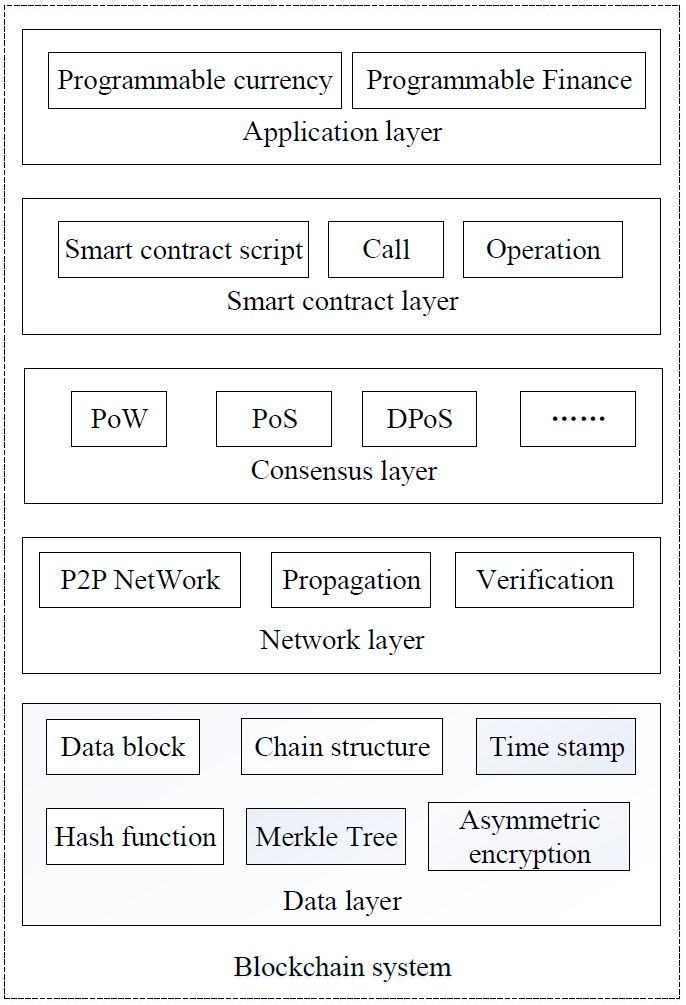
\includegraphics[width=\linewidth]{blockchain-layers}
    \caption{Blockchain infrastructure, from \cite{Duan2018}}
    \Description{Ilustration of the layers that describe a blockchain system}
    \label{fig:blockchain-layers}
  \end{figure}

The data layer is responsible for block generation, the construction of the blockchain and storage~\cite{Duan2018}. 
The network layer connects the data and filters packets, and also manages the nodes. 
The rules of how the blockchain protocol must work are defined on the consensus layer. 
This includes agreement between nodes, fault tolerance and data consistency. 
Smart contracts have their execution lifecycle on the smart contact layer.
The application layer is the upper level layer of used applications such as games or decentralized financial services. 

It is possible to use languages to define the standards of a blockchain system with mathematical rigor.
One of them is SDL (Specification and Description Language), an Object-Oriented formal language defined by the International Telecommunications Unit.
It is capable of mathematically describing the structure, behavior, and data of real-time and distributed communicating systems. 
It is also used by IEEE for standard definition~\cite{Duan2018}.

With SDL, we can describe a structure at the levels of system, block or process. A system represents the object to describe. 
It is responsible for the communication with the outer environment through the appropriate channels.
A system can contain one or more blocks and blocks contain one or more processes.
The majority of the functionality of an SDL system is described on the process level.
Comparing to conventional programming languages, modules are represented by blocks in SDL, and funcionalities are represented by processes.
In~\cite{Duan2018}, the authors propose a hierarchical model focused on the consensus layer.

  \subsection{Data Structure}
  In~\cite{Duan2018} the modelled blockchain system used an Improved Byzantine Fault Tolerant Algorithm as the consensus algorithm.
  To define the data structure of a block in SDL, we need to represent them as a pair with a header BT and body BH, where:

  \begin{displaymath}
    B~\equiv(B_H,B_T) \quad \textrm{with} \quad B_H~\equiv(\mathbb{H}_p,\mathbb{H}_a,\mathbb{H}_t,\mathbb{H}_m,\mathbb{H}_h) 
  \end{displaymath}
  \begin{displaymath}
    \quad \textrm{and} \quad B_T~\equiv(T_1,T_2,...,T_{\mathbb{H}_l}) 
  \end{displaymath}
  \linebreak[1]

  In these expressions, $\mathbb{H}_p$ represents the hash value of the previous block, 
  $\mathbb{H}_p$ the hash value of the current block, $\mathbb{H}_t$ it's timestamp, 
  $\mathbb{H}_m$ the merkle tree root (the hash of the transactions of a block), and $\mathbb{H}_h$ the current block's height.

  The the block' structure definition can be seen on Listing~\ref{lst:block-code}.
  
  \begin{lstlisting}[frame=single,label={lst:block-code},
    caption={Definition of a block's structure},captionpos=b, basicstyle=\ttfamily]
    newtype blockchain struct
      prehash integer;
      hash integer;
      length integer;/*the length of blocks*/
      merkleroot integer;
      ti Time;/*Timestamp*/
      translist list;
    endnewtype;

    newtype list
     array(maxit, integer)
    endnewtype;
 
    syntype maxit =Integer constants 0:25
    endsyntype;
  \end{lstlisting}
  
  A blockchain can be regarded as a state machine~\cite{Duan2018} that contains a starting state, a non-empty state, the input transaction set,
  a state transition function, and an acceptance state set. Which can be formally defined as:
    \begin{displaymath}
      S~\equiv(Q,\Sigma,\delta,s,F)
    \end{displaymath}

  Where:

  \begin{enumerate}
    \item[$\blacksquare$] Q is the non-empty state set, which represents all the states.
    \item[$\blacksquare$] $\Sigma$ is the set of the newly generated and consensus blocks. 
    \item[$\blacksquare$] $\delta$ represents the state transition function,
      \begin{math}
        \delta: Q \times \Sigma \rightarrow Q
      \end{math}.
    \item[$\blacksquare$] s would be the starting state, which is the state of the system when it initializes.
      \begin{math}
        \delta: s \in Q
      \end{math}.
    \item[$\blacksquare$] F representes the acceptance state set.
      \begin{math}
        F \subseteq Q
      \end{math}.
  \end{enumerate}
  \  \\ %fake break line
  The state of the model at the first block generation is the starting state.
  As transactions are made, the model a leader node to generate the block, which is transmitted to the other nodes on the blockchain network,
  triggering its validation for consensus. 
  A consensus block stores the hash of the previous one and adds it to the end of the blockchain and completes the transfer of the blockchain state.
  
  \subsubsection{Diagrams}
  With a modeling language like SDL, we can use diagrams to define blockchain structural entities, like the core system of the consensus layer
  and blocks. Process flowcharts can model the flow of information and input validation, making a process like
  node validations of blocks and its subprocess of synchronization and voting can clearly illustrated.

\section{Consensus Rule}\label{consensusRule}
Blockchain system may choose to use consensus rules taken from popular protocols such as Bitcoin,
but an alternative rule can be implemented, and also be formally modelled~\cite{Kawahara2020}.

On a consensus rule, fault tolerances requirements are of utmost importance, including the collusion of nodes to alter a ledger.
In~\cite{Kawahara2020}, the author discusses a way to formally describe these tolerances with a scalable verification.

Endorsement policies, the rule that define the criteria of agreement os transaction results between nodes, can be described
as a threshold function as follows:

\begin{displaymath}
  T(m,\textrm{node}_1,... ,\textrm{node}_n), m \in \mathbb{N}
\end{displaymath}
\linebreak[1]

Where $T(2,\textrm{node}_1,\textrm{node}_2,\textrm{node}_3)$ would be an endorsement policy
that means "among the three nodes in the argument, at least two nodes must return the same execution result".
With this, we can mathematically model faulty state verification.

\subsection{Faulty States}
Let $\mathbb{B}$ and $\mathbb{N}$ be sets of Boolean and natural numbers, respectively. The state of the \textit{i}-th node can be defined as:
$s_i = (s_i.e,s_i.v)$, where for each transaction execution, $s_i.e \in \mathbb{B}$ is the  existence of the result,
and $s_i.v \in \mathbb{B}$ is the value of the result (correct or wrong).

Using the threshold function previously shown, $T(m,s_1,... ,s_n) = (T.e,T.v)$. With this, let

\begin{displaymath}
  H_ = \left(\sum_{i}^{n} I(s_i.e \wedge (s_i.v = b)) \geq m \right)
\end{displaymath}

Where:

\begin{enumerate}
  \item[$\blacksquare$] \textit{m} is a threshold
  \item[$\blacksquare$] $b \in \mathbb{B}$
  \item[$\blacksquare$] $I : \mathbb{B} \mapsto \{0,1\}$  is the indicator function
\end{enumerate}
\  \\ %fake break line

With the expression above, the author of~\cite{Kawahara2020} infers:

\begin{displaymath}
  T.e = H_{\textrm{true}} \vee H_{\textrm{false}}, \quad T.v = \neg{H_{\textrm{false}}}
\end{displaymath}
\linebreak[1]

The  endorsement policy $EP = (EP.e,EP.v)$ can be formed with \textit{T}. When $EP.e = \textrm{true}$, the policy
is considered accordingly followed and the involved ledger is updated with the value of $EP.v$.

Mathematical descriptions like the ones above can also be applied to the fault tolerance of organizations participating in the blockchain in question.
With formal modeling, a consensus rule can be tested and benchmarked after giving the test case some arbitrary requirements that are in conformity with the scope.
The test results are used to judge the viability and scalability of the rule. 

\section{Smart Contracts}\label{smartContracts}
Smart contracts are the backend code of decentralized applications that live in blockchains such as Ethereum. 
This code cannot be changed once it is deployed to a production Net, so quality must be assured in order to guarantee
that specifications are followed and that vulnerabilities are inexistent~\cite{Murray2019}.
With the logic and mathematical modeling of formal verification, we avoid edge test cases that involve unforeseen inputs or conditions.

A smart contract's execution after its required verifications originates a transfer on a blockchain. Ethereum is a blockchain system
that allows is to deploy decentralized applications based on smart contracts, which are written in Solidity~\cite{Murray2019}.
Solidity has a limitation that makes smart contracts have a no parameters, no return value \textit{function()} that is anonymous
and defined as the fallback function~\cite{Liu2019}. When a contract sends Ether (the Ethereum blockchain token) but does not
not call any function, the fallback function is called. If this function does not exist int he contract, the transaction is cancelled.
This limitation can be used by hackers to exploit the contract, like the DAO smart contract exploit in 2016~\cite{Liu2019}.

A formal verification method using CPN modeling is proposed in~\cite{Liu2019}. In a scenario where a crowd funding smart contract (CFD) is considered, \cite{Liu2019} proposes a two layers contract modeling, 
the CFD layer model that establishes the overall structure of the contract, and a bottom layer that contains the AddTo layer
and the WithDraw layer, which implement deposit and withdrawing functions.
\begin{figure}[h]
  \centering
  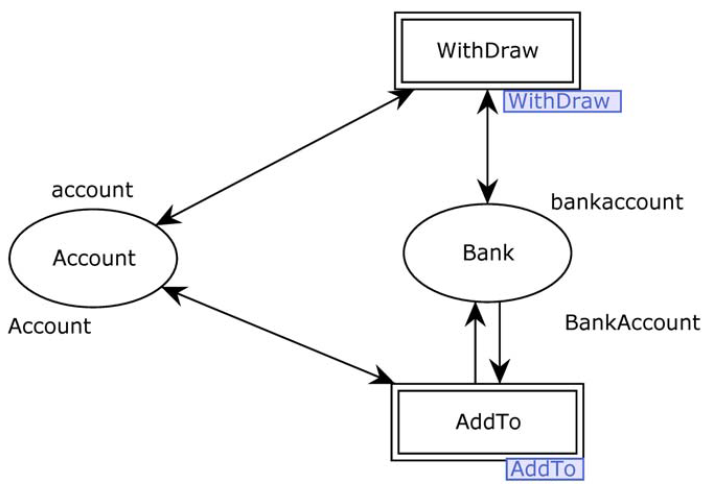
\includegraphics[width=\linewidth]{cfd-layer}
  \caption{CFD Layer, from \cite{Liu2019}}
  \Description{Ilustration of the layers that describe a blockchain system}
  \label{fig:cfd-layer}
\end{figure}

The CFD layer, shown on Figure~\ref{fig:cfd-layer}, presents the entity Account, that represents the user, Bank that represent
the contract account, and Withdraw and AddTo, that represent withdrawing and depositing operations.

\begin{figure}[h]
  \centering
  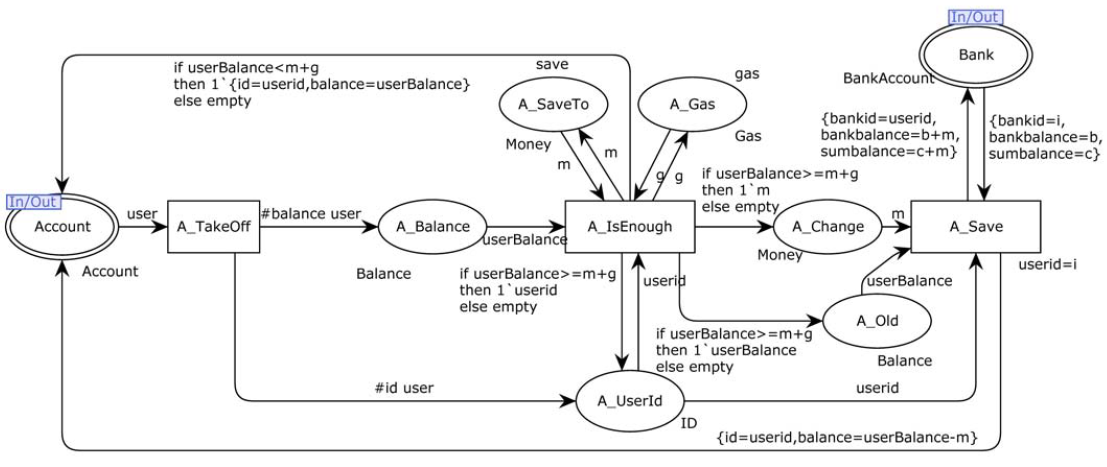
\includegraphics[width=\linewidth]{add-to-layer}
  \caption{AddTo Layer, from \cite{Liu2019}}
  \Description{Ilustration of the layers that describe a blockchain system}
  \label{fig:add-to-layer}
\end{figure}

The AddTo layer, shown on Figure~\ref{fig:add-to-layer}, models the user's depositing operations, where there are 
3 transactions and 8 entities in the model that describe the steps of a given transaction in the blockchain and it's conditions.

A similar to the on seen on Figure~\ref{fig:add-to-layer} was also presented in~\cite{Liu2019} for the WithDraw layer to describe the inherent processes
of withdraw operations and all their conditions.

Models like the proposed CPN model can be tested for resilience against malicious behavior using another model that attempts to exploit
the CFD contract. We can plan our attack model to test any operation and condition, such as balance altering, assurance of reception of funds,
etc. Smart contract's vulnerabilities can be taken advantage of by regular users executing expected operations, not only by badly intended actors 
with knowledge in computer science,~so it makes sense that scenarios of no attack can also be part of the model checking. 
CPN tools like Space State Tools can used to see the status of each step of a contract's execution during a test scenario~\cite{Liu2019},
easing the discovert of vulnerabilities.

\section{Security}\label{security}
As mentioned in section~\ref{formalModeling}, formal analysis and verification is used to assure security of a blockchain's core structures and consensus rule.
But we can cover the security-requirements for backend blockchain protocol and mechanisms to ensure the assumptions and scripting language~\cite{Matsuo2017}.

In~\cite{Matsuo2017}, the authors enumerate security requirements of a blockchain system by their layers, consisting of cryptography layer, backbone protocol, application protocol,
application logic, implementation and operation. These requirements can be seen in Table~\ref{tab:security-layers}.

  \begin{table}
    \caption{Blockchain Technology layers and security considerations}
    \label{tab:security-layers}
    \begin{tabularx}{\linewidth}{ccl}
      \toprule
      Layer&Security Consideration& Standard \\
      \toprule
      Operation & \makecell{Key Management, \\Audit, Backup} & ISO/IEC 27000 \\ 
      \midrule
      Implementation & \makecell{Program Code,\\Secure Hardware} & ISO/IEC 15408 \\ 
      \midrule
      Application Logic & \makecell{Scripting Language\\for Financial\\Transaction,\\ Contract} & \makecell{Secure coding\\guides} \\ 
      \midrule
      Application Protocol & \makecell{Privacy protection,\\Secure transaction} & ISO/IEC 29128 \\ 
      \midrule
      Backbone Protocol & \makecell{PSP, Consensus,\\Merkle Tree} & ISO/IEC 29128 \\ 
      \midrule
      Cryptography & \makecell{ECDSA, SHA-2,\\RIPEMD160} & NIST, ISO \\
      \bottomrule
  \end{tabularx}
  \end{table}

We can implement formal methods in the layers Implementation, Backbone protocol, Application protocol and Language for Smart Contract.
In the implementation layer we have both software and hardware implementation pf security mechanisms, including the cryptographic algorithm,
protocols and key management mechanisms. In the Backbone protocol and application protocol deals with cryptographic protocols.
The security of the source code of a smart contracts are also mention in~\cite{Matsuo2017}, which can be modeled and verified according to requirements,
as shown in section~\ref{smartContracts}.

%%
%% The next two lines define the bibliography style to be used, and
%% the bibliography file.
\bibliographystyle{ACM-Reference-Format}
\bibliography{article-base}


\end{document}
\endinput
%%
%% End of file `article.tex'.
